% This is "sig-alternate.tex" V2.1 April 2013
% This file should be compiled with V2.8 of "sig-alternate.cls" May 2012
%
% This example file demonstrates the use of the 'sig-alternate.cls'
% V2.8 LaTeX2e document class file. It is for those submitting
% articles to ACM Conference Proceedings WHO DO NOT WISH TO
% STRICTLY ADHERE TO THE SIGS (PUBS-BOARD-ENDORSED) STYLE.
% The 'sig-alternate.cls' file will produce a similar-looking,
% albeit, 'tighter' paper resulting in, invariably, fewer pages.
%
% ----------------------------------------------------------------------------------------------------------------
% This .tex file (and associated .cls V2.8) produces:
%       1) The Permission Statement
%       2) The Conference (location) Info information
%       3) The Copyright Line with ACM data
%       4) NO page numbers
%
% as against the acm_proc_article-sp.cls file which
% DOES NOT produce 1) thru' 3) above.
%
% Using 'sig-alternate.cls' you have control, however, from within
% the source .tex file, over both the CopyrightYear
% (defaulted to 200X) and the ACM Copyright Data
% (defaulted to X-XXXXX-XX-X/XX/XX).
% e.g.
% \CopyrightYear{2007} will cause 2007 to appear in the copyright line.
% \crdata{0-12345-67-8/90/12} will cause 0-12345-67-8/90/12 to appear in the copyright line.
%
% ---------------------------------------------------------------------------------------------------------------
% This .tex source is an example which *does* use
% the .bib file (from which the .bbl file % is produced).
% REMEMBER HOWEVER: After having produced the .bbl file,
% and prior to final submission, you *NEED* to 'insert'
% your .bbl file into your source .tex file so as to provide
% ONE 'self-contained' source file.
%
% ================= IF YOU HAVE QUESTIONS =======================
% Questions regarding the SIGS styles, SIGS policies and
% procedures, Conferences etc. should be sent to
% Adrienne Griscti (griscti@acm.org)
%
% Technical questions _only_ to
% Gerald Murray (murray@hq.acm.org)
% ===============================================================
%
% For tracking purposes - this is V2.0 - May 2012

\documentclass{sig-alternate}

\setlength{\paperheight}{11in}
\setlength{\paperwidth}{8.5in}
\usepackage[
  pass,% keep layout unchanged
  % showframe,% show the layout
]{geometry}

\begin{document}

% Copyright
\setcopyright{waclicense}


%% DOI
%\doi{10.475/123_4}
%
%% ISBN
%\isbn{123-4567-24-567/08/06}
%
%%Conference
\conferenceinfo{Web Audio Conference WAC-2022,}{December 6--8, 2022, Cannes, France.}
\CopyrightYear{2022} % Allows default copyright year (20XX) to be over-ridden - IF NEED BE.
%\crdata{0-12345-67-8/90/01}  % Allows default copyright data (0-89791-88-6/97/05) to be over-ridden - IF NEED BE.
% --- End of Author Metadata ---

\title{TimeSide API as an audio processing web service}
%\subtitle{[Extended Abstract]
%\titlenote{A full version of this paper is available as
%\textit{Author's Guide to Preparing ACM SIG Proceedings Using
%\LaTeX$2_\epsilon$\ and BibTeX} at
%\texttt{www.acm.org/eaddress.htm}}}
%
% You need the command \numberofauthors to handle the 'placement
% and alignment' of the authors beneath the title.
%
% For aesthetic reasons, we recommend 'three authors at a time'
% i.e. three 'name/affiliation blocks' be placed beneath the title.
%
% NOTE: You are NOT restricted in how many 'rows' of
% "name/affiliations" may appear. We just ask that you restrict
% the number of 'columns' to three.
%
% Because of the available 'opening page real-estate'
% we ask you to refrain from putting more than six authors
% (two rows with three columns) beneath the article title.
% More than six makes the first-page appear very cluttered indeed.
%
% Use the \alignauthor commands to handle the names
% and affiliations for an 'aesthetic maximum' of six authors.
% Add names, affiliations, addresses for
% the seventh etc. author(s) as the argument for the
% \additionalauthors command.
% These 'additional authors' will be output/set for you
% without further effort on your part as the last section in
% the body of your article BEFORE References or any Appendices.

\numberofauthors{4} %  in this sample file, there are a *total*
% of EIGHT authors. SIX appear on the 'first-page' (for formatting
% reasons) and the remaining two appear in the \additionalauthors section.
%
\author{
% You can go ahead and credit any number of authors here,
% e.g. one 'row of three' or two rows (consisting of one row of three
% and a second row of one, two or three).
%
% The command \alignauthor (no curly braces needed) should
% precede each author name, affiliation/snail-mail address and
% e-mail address. Additionally, tag each line of
% affiliation/address with \affaddr, and tag the
% e-mail address with \email.
%
% 1st. author
\alignauthor
       \name{Guillaume Pellerin}
       \affaddr{IRCAM, Paris}
       \email{pellerin@ircam.fr}
% 2nd. author
\alignauthor
       \name{Paul Brossier}
       \affaddr{Aubio}
       \email{piem@piem.org}
\and       
% 4th. author
\alignauthor
       \name{Martin Desrumaux}
       \affaddr{IRCAM, Paris (until 2022)}
       \email{martin@letik.io}
% 3rd. author
\alignauthor
       \name{Antoine Grandry}
       \affaddr{IRCAM, Paris (until 2020)}
       \email{antoine.grandry@hotmail.fr}
}

\date{22 April 2022}
% Just remember to make sure that the TOTAL number of authors
% is the number that will appear on the first page PLUS the
% number that will appear in the \additionalauthors section.

\maketitle
\begin{sloppypar}
\begin{abstract}
Audio descriptors can help to analyze, classify and compare sounds by their own characteristics. For large datasets, it is often needed to store the results of the analyses in order to keep everything sustainable and comparable, especially in machine learning usecases. This demo will show how to use the TimeSide REST API as a remote service to process descriptors in order to embed the results in any web application. The new version of the TimeSide player will be presented as a general example of using the dedicated javascript SDK to produce new kinds of applications involving visualization and collaborative annotation.
\end{abstract}


%
% The code below should be generated by the tool at
% http://dl.acm.org/ccs.cfm
% Please copy and paste the code instead of the example below.
%
%\begin{CCSXML}
%<ccs2012>
 %<concept>
  %<concept_id>10010520.10010553.10010562</concept_id>
  %<concept_desc>Computer systems organization~Embedded systems</concept_desc>
  %<concept_significance>500</concept_significance>
 %</concept>
 %<concept>
  %<concept_id>10010520.10010575.10010755</concept_id>
  %<concept_desc>Computer systems organization~Redundancy</concept_desc>
  %<concept_significance>300</concept_significance>
 %</concept>
 %<concept>
  %<concept_id>10010520.10010553.10010554</concept_id>
  %<concept_desc>Computer systems organization~Robotics</concept_desc>
  %<concept_significance>100</concept_significance>
 %</concept>
 %<concept>
  %<concept_id>10003033.10003083.10003095</concept_id>
  %<concept_desc>Networks~Network reliability</concept_desc>
  %<concept_significance>100</concept_significance>
 %</concept>
%</ccs2012>
%\end{CCSXML}
%
%\ccsdesc[500]{Computer systems organization~Embedded systems}
%\ccsdesc[300]{Computer systems organization~Redundancy}
%\ccsdesc{Computer systems organization~Robotics}
%\ccsdesc[100]{Networks~Network reliability}
%
%
%%
%% End generated code
%%
%
%%
%%  Use this command to print the description
%%
%\printccsdesc
%
%% We no longer use \terms command
%%\terms{Theory}
%
%\keywords{ACM proceedings, \LaTeX, text tagging}


\section{Introduction}

As the number of online audio applications and datasets increase, it becomes crucial for researchers and engineers to be able to prototype and test their own algorithms as fast as possible on various platforms and usecases like computational musicology\cite{fillon2017wac} and streaming services. On the other side, content providers and producers need to enhance user experiences on their platforms with more metadata based on cultural history but also audio feature analyses. Growing those metadata synchronously with the music published on the internet implies that the analysis and storage systems can be easily updated, scaled and deployed.

TimeSide\cite{timesiderepo} has been developed in this sense to propose an online audio processing service. It provides a REST API as well as a javascript SDK so that web developers can easily embed the service into their own applications without requesting to much local resources on the user side to compute audio features\cite{buffa2021wasabi}\cite{buffa:hal-02366730}.

We will show in this demo how to use the SDK and consume the API in various web oriented contexts. As a first example, the new TimeSide Player prototype will be presented.

\section{TimeSide Core Framework}

TimeSide is first a python framework enabling low and high level audio analysis, imaging, transcoding, streaming and labelling. Its high-level API is designed to enable complex processing on very large datasets of any audio or video assets with a plug-in architecture, a secure scalable backend and an extensible dynamic web frontend. Some usecases: scaled audio computing (filtering, machine learning, etc), web audio visualization, audio process prototyping, realtime and on-demand transcoding and streaming over the web, automatic segmentation and labelling synchronized with audio events

Because there are a lot of tools available in the Python ecosystem dedicated to music information retrieval, machine learning and data analysis, we have decided to embed all main ones: Aubio\cite{aubio}, Yaafe\cite{yaafe_ISMIR2010}, Essentia\cite{essentia}, VAMP\cite{vamp-plugins}, librosa\cite{librosa}, GStreamer, TensorFlow, Torch, PyTorch, scikit-learn, Jupyter, Pandas and Pytables. They are used to develop native TimeSide plugins though its simple processing API.

\section{TimeSide REST API}

In addition to be usable as a library, TimeSide has furthermore been built into a Django server with a relational PostgreSQL database in order to store music tracks and processing results. Data structure and relations are defined in the models to ensure easy data serialization. The backend is built with Django REST Framework\cite{drf} to provide a documented RESTful API\cite{timesideapidoc}. It guarantees interoperability by allowing other servers or multiple frontends to interact with the TimeSide instance. Any application consuming the API is then able to: upload audio track or retrieve them from remote providers, stream original or transcoded sources, run on-demand analysis with customized parameters, deliver and share several types of results: transcoded audio, numerical or graphical outputs of analysis, collect tags and indices on tracks to build annotated audio corpora for further machine learning purpose\cite{peeters2012towards}.


\section{TimeSide Javascript SDK}
 A  (SDK) is also available to help . An example of its use - an augmented HTML5 player - is discussed in next section. 
 
In order to build frontends on top of this web API, a Software Development Kit (SDK) is available\cite{timesidesdk} for the Javascript and Typescript languages. It has been created from the  routes of the OpenAPI schema automatically exported from the backend thanks to the OpenAPI Generator\cite{openapigenerator}. The SDK proposes  some examples for clients to reach the server and request some processing.


\section{TimeSide Player}

The previous versions of the player was consuming the data processed and rendered by the backend only as bitmap images. This would avoid to zoom in very little scales\cite{fillon2017wac}. As the REST API gives now the possibility to stream the processing results directly from the database into the browser as vectorized data, we have rebuild the entire interface to display the features  through a dynamic multi-track interface based on D3.js\cite{d3js} and VueJS. An annotation system also allows to describe an audio event between two times on each track so that users can show and share their analyses in a collaborative way. This open a lot of new usecases between sound and music  databases and citizen science protocols.

\begin{figure}[!h]
    \centering
    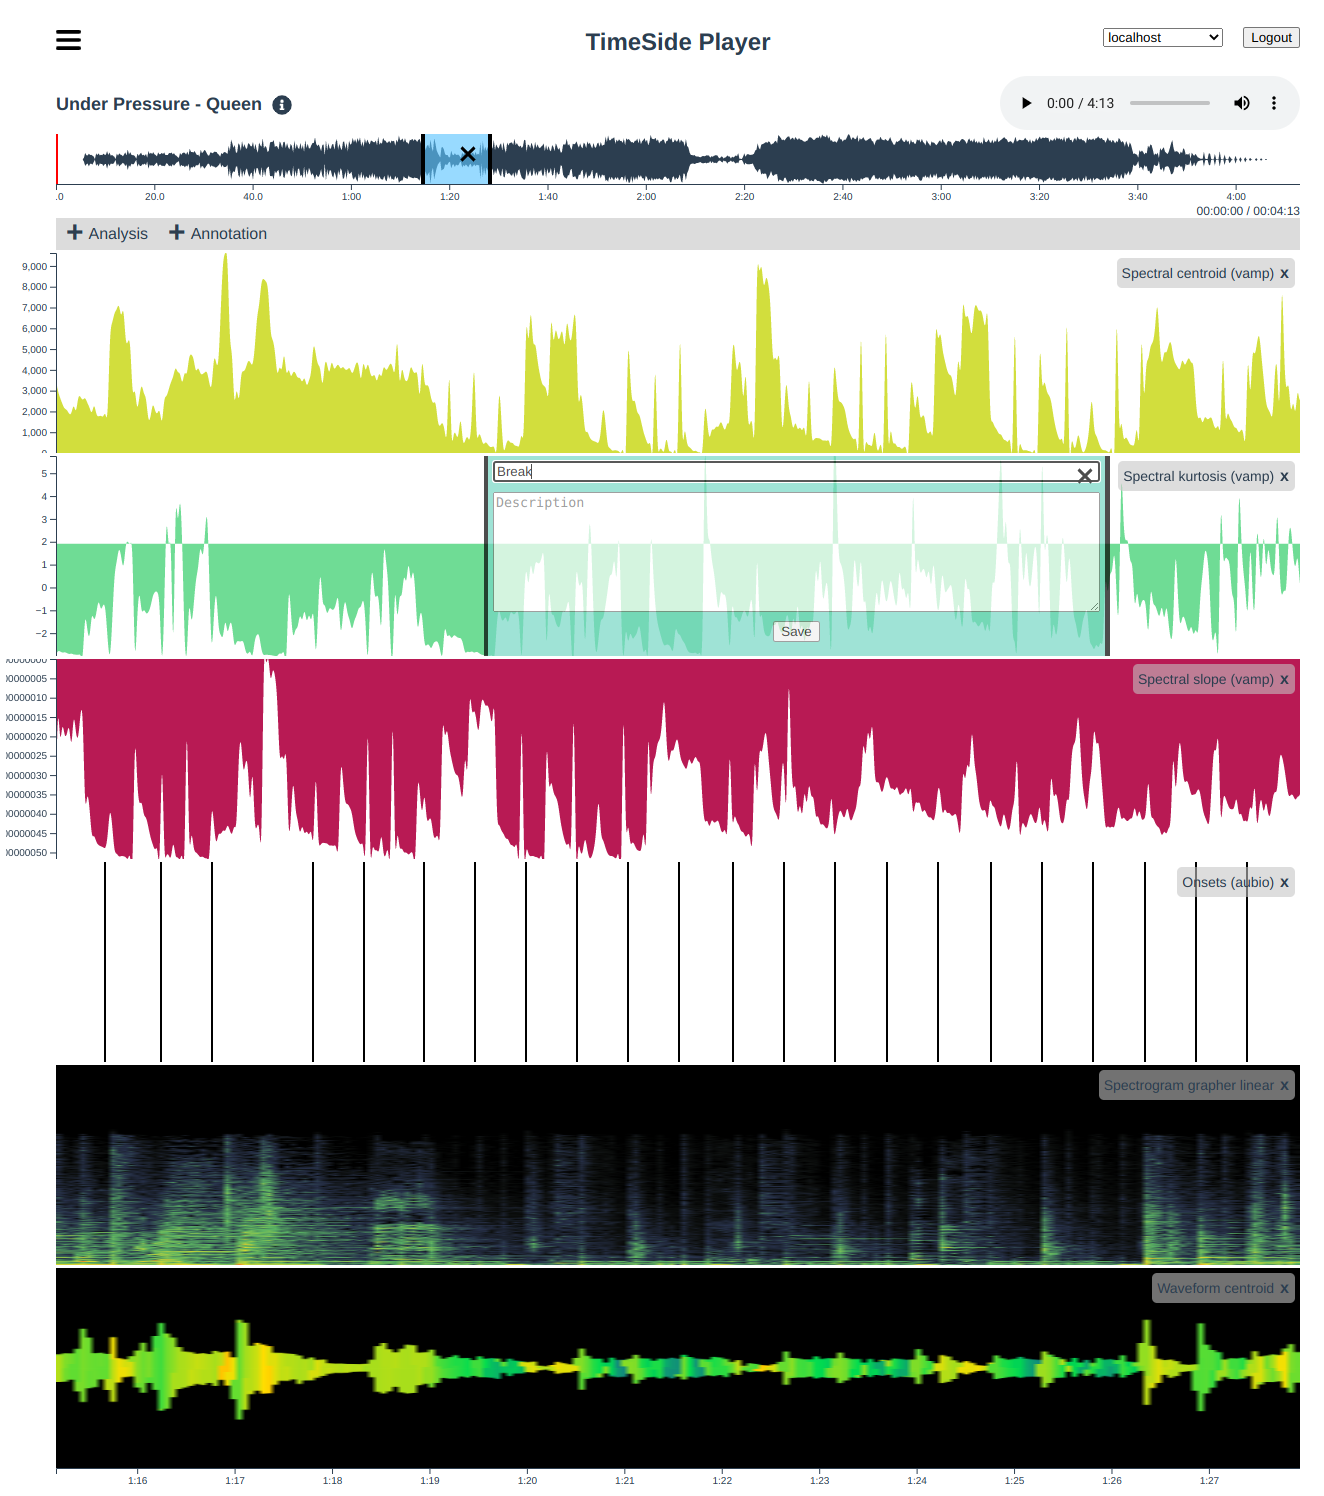
\includegraphics[width=\linewidth]{figures/timeside-player-wac-22.png}
    \caption{Overview of the Timeside-Player interface picturing timbre and rhythm analyses for the Queen song "Under Pressure". It shows (a) the audio player and various vectorized audio descriptors (Spectral centroid, Spectral kurtosis, Spectral slope, Onsets, Linear Spectrogram and Waveform) as well as the time annotation system.}
    \label{fig:timeside}
\end{figure}

\section{Demonstration}

We will show how to use the player as well as the SDK to interact with the web service requesting YouTube and Deezer track analyses.

\section{Technical requirements}

Only a computer, brought by the demonstrator, and a WiFi internet access are needed for this demonstration.

%ACKNOWLEDGMENTS are optional
\section{Acknowledgments}
This work was supported by the French Research National
Agency (ANR) and the WASABI team (contract
ANR-16-CE23-0017-01).

%
% The following two commands are all you need in the
% initial runs of your .tex file to
% produce the bibliography for the citations in your paper.
\bibliographystyle{abbrv}
\bibliography{wac2022}  % sigproc.bib is the name of the Bibliography in this case
% You must have a proper ".bib" file
%  and remember to run:
% latex bibtex latex latex
% to resolve all references
%
% ACM needs 'a single self-contained file'!
%
%APPENDICES are optional
%\balancecolumns
\end{sloppypar}
\end{document}
